\chapter[Cronograma]{Cronograma}
\label{chap:crono}

A Figura \ref{img:cronograma} mostra o cronograma das atividades realizadas durante a primeira parte do projeto.

\begin{figure}[H]
    \centering
    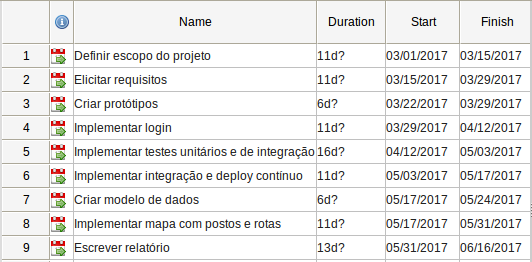
\includegraphics[scale=0.5]{figuras/cronograma_r1.png}
    \caption[Cronograma de atividades da primeira entrega.]{Cronograma de atividades da primeira entrega. Fonte: autores}
    \label{img:cronograma}
\end{figure}

A Figura \ref{img:cronograma2inicial} apresenta o cronograma inicial da segunda parte do projeto.

\begin{figure}[H]
    \centering
    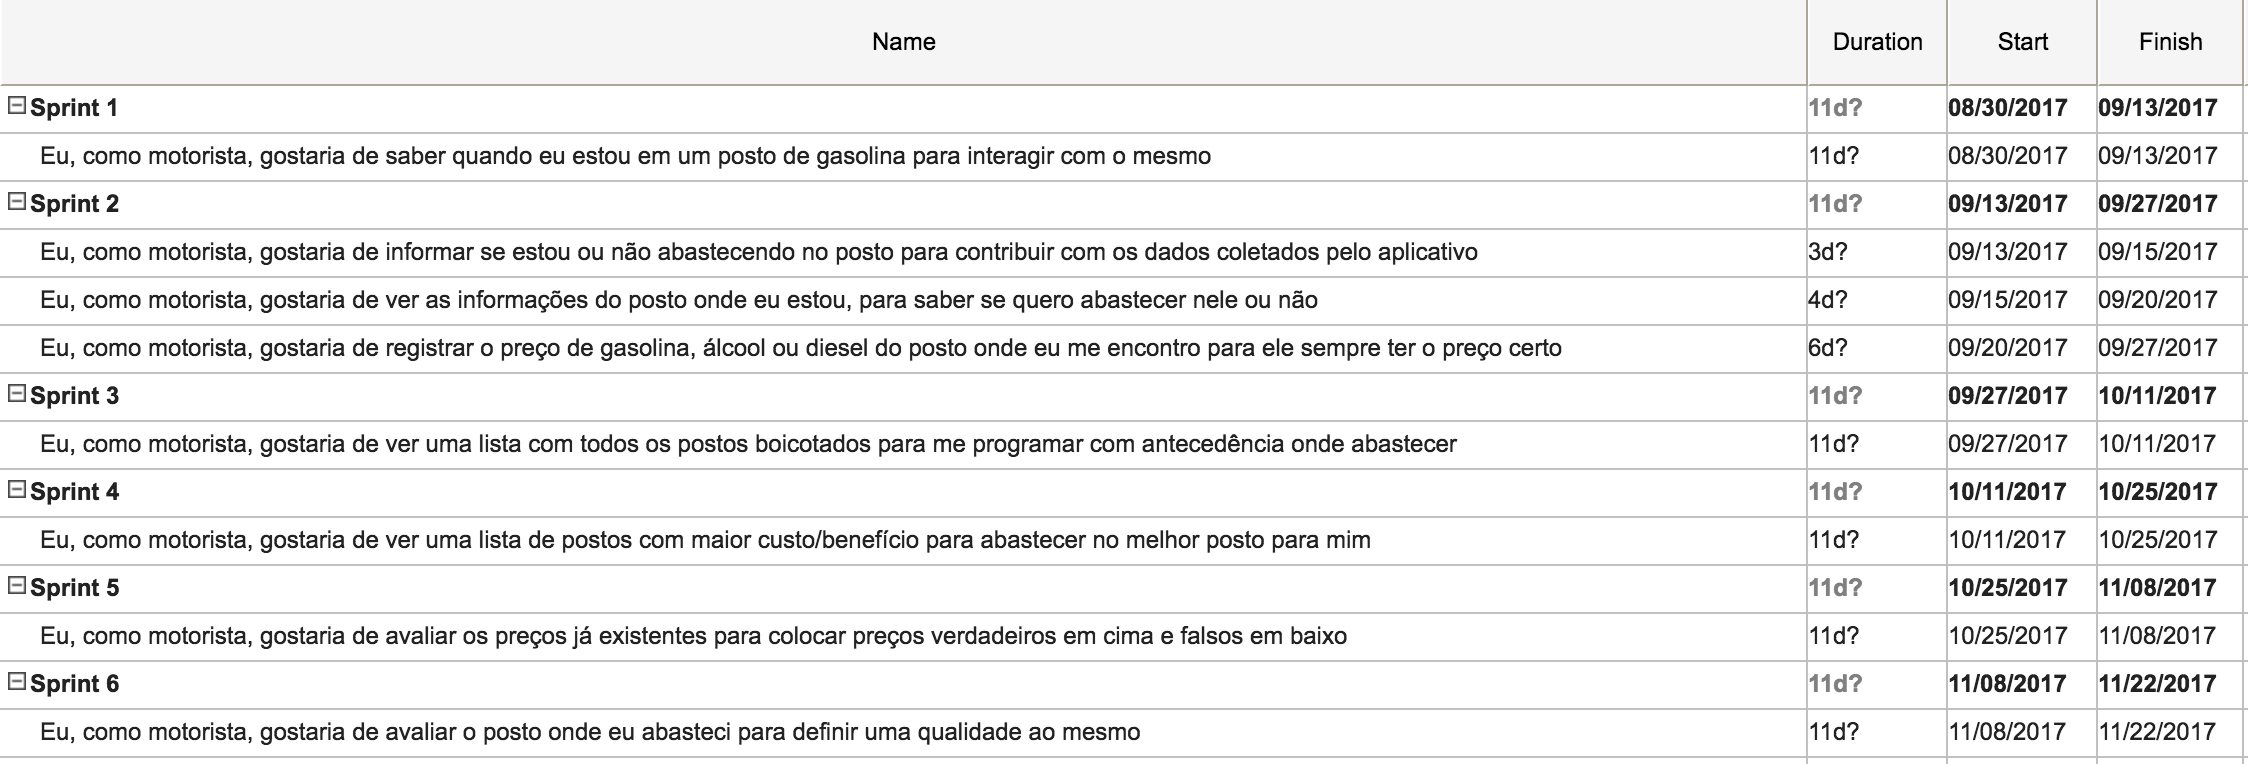
\includegraphics[scale=0.4]{figuras/cronograma_segunda_parte_1.png}
    \caption[Cronograma inicial de atividades da segunda entrega.]{Cronograma inicial de atividades da segunda entrega. Fonte: autores}
    \label{img:cronograma2inicial}
\end{figure}
\pagebreak

Porém, devido a certas adversidades e melhor compreensão do projeto, foram feitas certas mudanças no cronograma, como mostra a Figura \ref{img:cronogramafinal}.

\begin{figure}[H]
    \centering
    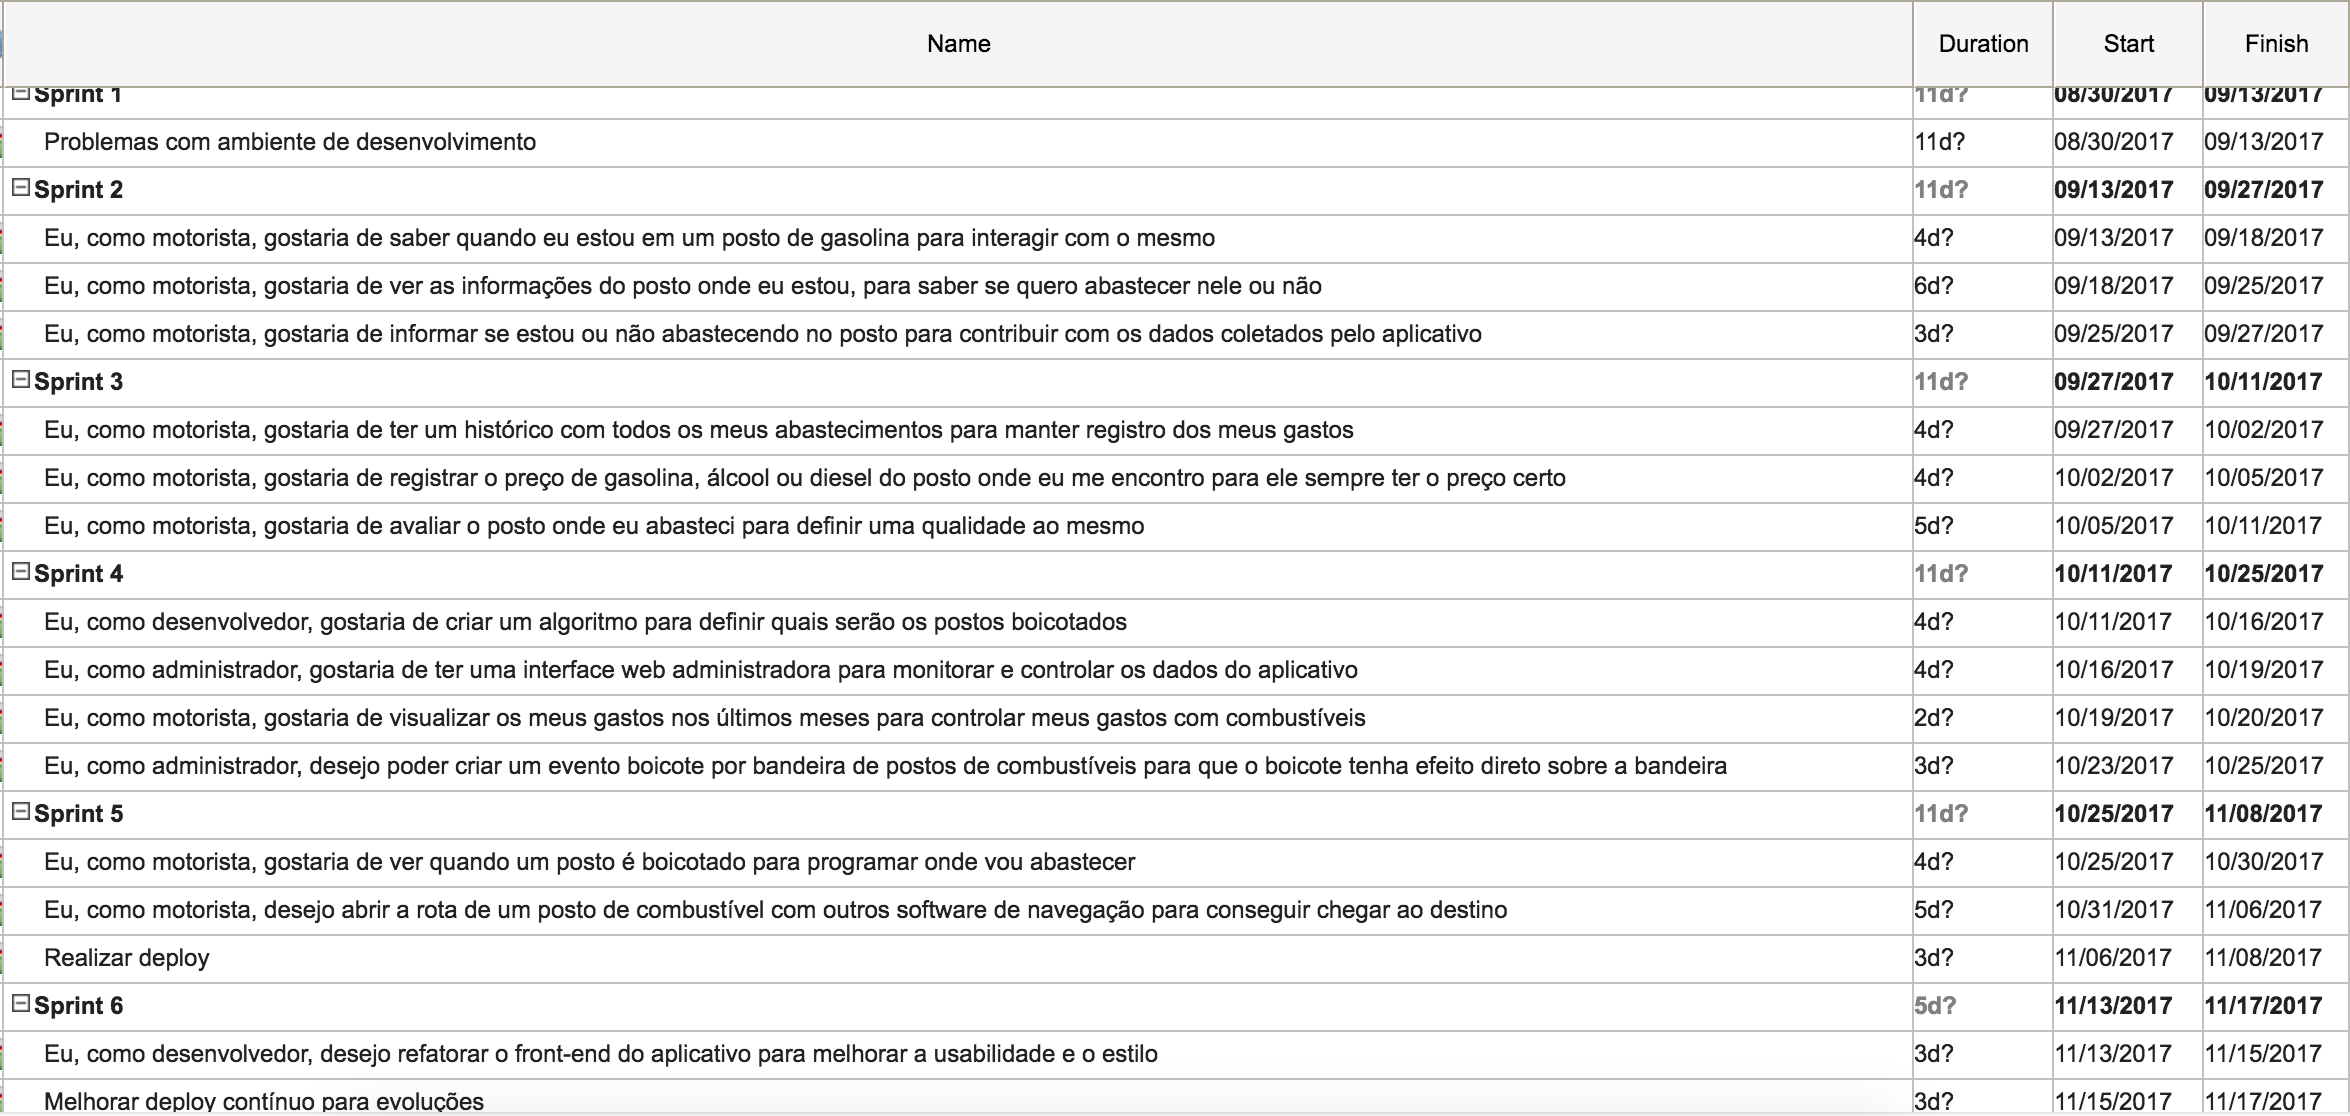
\includegraphics[scale=0.4]{figuras/cronograma_segunda_parte_2.png}
    \caption[Cronograma final de atividades da segunda entrega.]{Cronograma final de atividades da segunda entrega. Fonte: autores}
    \label{img:cronogramafinal}
\end{figure}

Principalmente na primeira \textit{sprint}, alguns problemas foram encontrados com o ambiente de desenvolvimento do Ionic devido à da atualização do Ionic 2 para o Ionic 3. A maioria dos problemas estavam relacionados a atualizações de dependências.

O \textit{plugin} do \textit{Geofence}, utilizado para definir cercas geográficas nos postos de combustível para indicar ao usuário quando ele entra em um posto, foi implementado para o iOS na linguagem de programação Swift. A Apple atualizou o Swift da versão 2 para a versão 3 durante o desenvolvimento, mas o \textit{plugin} ainda não foi atualizado, o que gerou incompatibilidade do serviço oferecido pelo \textit{plugin} com a plataforma iOS. Mesmo depois de muitas tentativas de fazê-lo funcionar nesta plataforma, não foi obtido êxito. Portanto, a equipe de desenvolvimento, juntamente com o professor orientador, tomaram a decisão de pausar o desenvolvimento para a plataforma iOS e focar apenas para a plataforma Android, evitando assim que todo o trabalho fosse prejudicado pela atualização de uma dependência que ainda não ocorreu.

Além do problema da plataforma da Apple, apesar do \textit{plugin} \textit{Geofence} ter suporte para notificações \textit{push} (mensagens de alerta enviadas para o usuário notificando na tela do aparelho) locais, uma opção para facilitar a escalabilidade do aplicativo, caso seja necessário enviar notificações \textit{push} em outros momentos, é a utilização de algum serviço externo para enviar as notificações. Essa decisão causou novos atrasos na implementação da funcionalidade, pois foi necessário realizar pesquisas sobre novas alternativas. Por fim, foi utilizado o serviço de notificações \textit{push} do Google, o Firebase.

Durante a sprint 4, percebeu-se que seria necessário uma tela de administração para poder definir os ícones dos postos, bem como corrigir quaisquer informações incorretas oriundas das fontes externas, o que justifica sua adição ao cronograma. Durante a mesma sprint, viu-se necessário melhorar a interface do aplicativo pois o foco até então havia sido exclusivamente em desenvolver as funcionalidades. Porém, essa melhoria foi alocada para a sprint 6 porque a sprint 4 e a sprint 5 já possuíam muitas tarefas.
